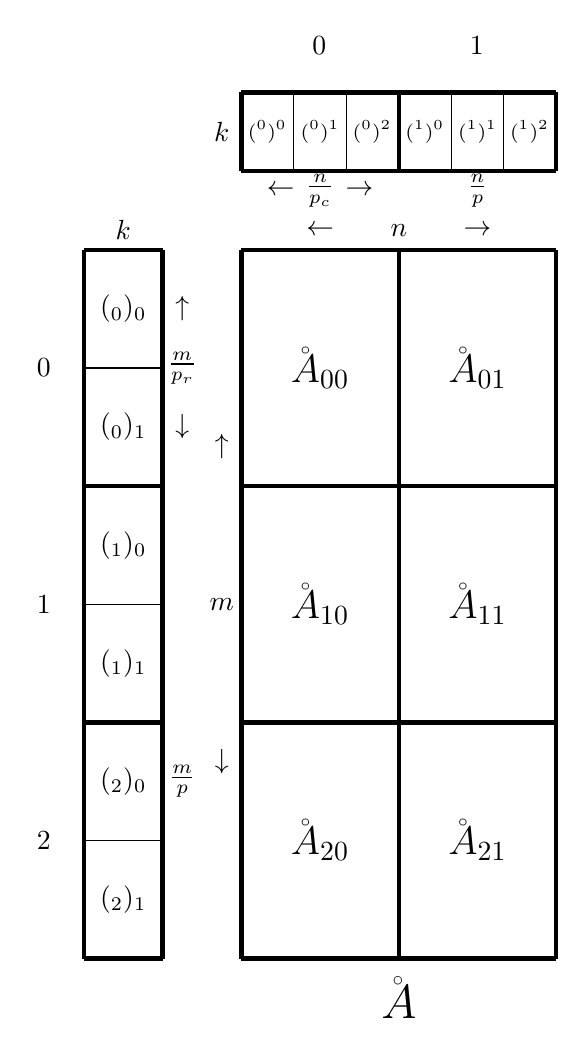
\begin{tikzpicture}

%% draw matrix distributions with scaled grids
% A
\draw[xscale=2,yscale=3,ultra thick] (0,0) grid (2,3);
% W
\draw[yscale=3/2] (-2,0) grid (-1,6);
\draw[yscale=3,ultra thick] (-2,0) grid (-1,3);
% H
\draw[xscale=2/3] (0,10) grid (6,11);
\draw[xscale=2,ultra thick] (0,10) grid (2,11);

%% add (sub)matrix names 
% A
\node[draw=none] at (2,-0.5) {\LARGE $\AA$};
\node[draw=none] at (1,7.5) {\Large $\AA_{00}$};
\node[draw=none] at (1,4.5) {\Large $\AA_{10}$};
\node[draw=none] at (1,1.5) {\Large $\AA_{20}$};
\node[draw=none] at (3,7.5) {\Large $\AA_{01}$};
\node[draw=none] at (3,4.5) {\Large $\AA_{11}$};
\node[draw=none] at (3,1.5) {\Large $\AA_{21}$};
% W
\node[draw=none] at (-1.5,-0.5) {\LARGE $\WW$};
\node[draw=none] at (-2.5,7.5) {\Large $\WW_0$};
\node[draw=none] at (-2.5,4.5) {\Large $\WW_1$};
\node[draw=none] at (-2.5,1.5) {\Large $\WW_2$};
\node[draw=none] at (-1.5,8.25) {$(\WW_0)_0$};
\node[draw=none] at (-1.5,6.75) {$(\WW_0)_1$};
\node[draw=none] at (-1.5,5.25) {$(\WW_1)_0$};
\node[draw=none] at (-1.5,3.75) {$(\WW_1)_1$};
\node[draw=none] at (-1.5,2.25) {$(\WW_2)_0$};
\node[draw=none] at (-1.5,0.75) {$(\WW_2)_1$};
% H
\node[draw=none] at (-1,10.5) {\LARGE $\HH$};
\node[draw=none] at (1,11.5) {\Large $\HH^0$};
\node[draw=none] at (3,11.5) {\Large $\HH^1$};
\node[draw=none] at (.33,10.5) {\scriptsize $(\HH^0)^0$};
\node[draw=none] at (1,10.5) {\scriptsize $(\HH^0)^1$};
\node[draw=none] at (1.66,10.5) {\scriptsize $(\HH^0)^2$};
\node[draw=none] at (2.33,10.5) {\scriptsize $(\HH^1)^0$};
\node[draw=none] at (3,10.5) {\scriptsize $(\HH^1)^1$};
\node[draw=none] at (3.66,10.5) {\scriptsize $(\HH^1)^2$};

% label vertical dimensions
\node[draw=none] at (-0.25,10.5) {$k$};
\node[draw=none] at (-0.25,4.5) {$m$};
\node[draw=none] at (-0.25,6.5) {$\uparrow$};
\node[draw=none] at (-0.25,2.5) {$\downarrow$};
\node[draw=none] at (-0.75,7.5) {$\frac{m}{p_r}$};
\node[draw=none] at (-0.75,8.25) {$\uparrow$};
\node[draw=none] at (-0.75,6.75) {$\downarrow$};
\node[draw=none] at (-0.75,2.25) {$\frac{m}{p}$};
% label horizontal dimensions
\node[draw=none] at (-1.5,9.25) {$k$};
\node[draw=none] at (2,9.25) {$n$};
\node[draw=none] at (1,9.25) {$\leftarrow$};
\node[draw=none] at (3,9.25) {$\rightarrow$};
\node[draw=none] at (1,9.75) {$\frac{n}{p_c}$};
\node[draw=none] at (0.5,9.75) {$\leftarrow$};
\node[draw=none] at (1.5,9.75) {$\rightarrow$};
\node[draw=none] at (3,9.75) {$\frac{n}{p}$};

\end{tikzpicture}